%!TEX root = ../report.tex

% 
% Architecture
% 

\section{Architecture (2/3pgs)}
\label{sec:arch}

The proposed solution covers three main problems previously identified in Rosetta's programming environment: (1) poor or non-existent context explanation, (2) invisible program flow and (3) non-existence of immediate feedback. The solution, of each one of these problems, are describe in a proper section. 

The following section present how these solutions are going to be combined. Additionally, what are the main quality attributes we seek for this solution.

\subsection{General Architecture}

The Figure~\ref{fig:sol}, represent the general architecture of the solution.

It is a typical repository style (see Section~\ref{sec:ide}), the proposed tools are represented by the rounded rectangle surrounding by two square rectangles, which means the repositories, or furthermore the tool input or output. The DrRacket repository will produce the \ac{ide} meta-data, e.g. symbol table, the \ac{ast}, etc, in the other hand, the Rosetta back-end will have the \ac{gd} data, for instance the geometric object locations. For example, the tool that implements the immediate feedback is constantly running the program in the \ac{ide} side, as a result it indirectly causes an effect at the Rosetta back-end.

The tools can be implemented separately, however is necessary to implement an exact data model required by the \ac{ide} and also by the back-end. In the \ac{ide} side, we will use the plug-ins to extend DrRacket functionality and in the Rosetta back-end we will use the existing communication protocol, since it has several back-ends. 


\begin{figure}[!htbp]
 \centering
 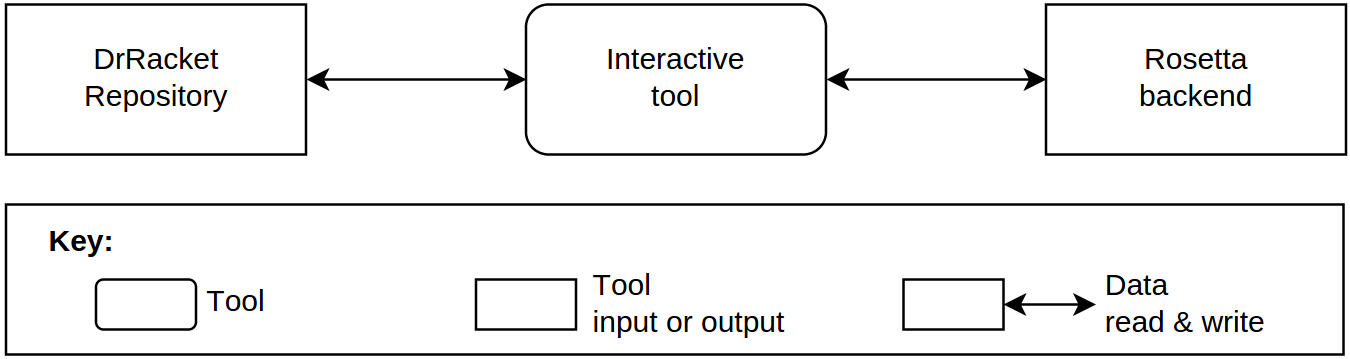
\includegraphics[scale=0.2]{img/sol}
 \caption{General architecture of the proposed interactive tools. On the right, the DrRacket~\ac{ide} as a shared data repository. On the left, the Rosetta back-end also as a repository of data. The tools, in the center, are interacting with the repositories.}
 \label{fig:sol}
\end{figure}

Before going through each tool, is important to define the quality attributes we are going to address. Mainly, we seek to achieve the following:

\begin{itemize}
 \item Interoperability. Actually, Rosetta has already achieved this quality. However, we want to improve it by tailoring as much as possible the DrRacket interface for a \ac{gd} system.
 
 \item Modifiability. Rosetta is a project been developed, thereby is necessary to be prepared for changes. For this, we have studied other kind of \ac{ide}s integration and new strategies to improve productivity.
 
 \item Performance. The interactiveness of the tools depend directly on the performance of the system. Since, the tools should respond in a very low latency, to be, indeed, interactive. Generally, \ac{gd} systems do not lead well with performance. As a result, new strategies should be thought. For example, the use of alternative back-ends, and also, using copies of computations, i.e. mechanisms of cache.  
 
 \item Security. Since in live programming the code is executed immediately, must be necessary a security mechanism. For example, our proposed solution is construct a sandbox, similar as used in PythonTutor.
\end{itemize}

\subsection{Explaining the context}

A programming environment for \ac{gd} systems, is a \ac{ui} for create models. Especially in these systems, where the elements of the program and those of the model are strongly related, the environment must be designed to explain this relationship. Since it is particularly important for program comprehension, maintenance, and debugging. The use of this ability, also known as traceability, allows designers understand faster the cause of errors, the changes to adapt a \ac{gd} program, as well as the impact of the changes to a program.

Several techniques have been applied, to improve traceability in \ac{gd}. In general, the traceability is just supported in one direction. For example, in Grasshopper and Dynamo, when a user selects a component that generates geometry, the corresponding part in the model is highlighted. However the inverse is not supported.

Rosetta has proposed the bi-directional traceability. Starting from the model, it is possible to point to some shape element and identify the part of the program that was responsible for its creation. Starting from the program, it is possible select the expressions and identify its generated model. However, before a user selecting an expression would be interesting that he knows its context, meaning, for instance, its parameters and its purpose in the code. For this, we suggest the traceability using sketches.

\subsubsection{Traceability with sketches}

Most architects before going to translate his models into a \ac{gd} tool, often write in a piece of paper a sketch that represent the future design, which may have a coherent parametrization. So, this design can be used to illustrate the code by taking the advantage provide by the DrRacket~\ac{ide}, which allows the inclusion of images in the code. The next steep is bind the parameters of the functions with the image symbols.


The Figure~\ref{fig:trace}, shows some advances in the direction of implementation. Those results, were obtained by using the syntax checker provided by DrRacket to annotate the source text, of syntactically correct programs. The syntax checker, marks up the source text based on five syntactic categories: primitives, keywords, bound variables, free variables, and constants. Thus, when the programmer move the mouse over an identifier, the syntax checker display arrows that point from bound identifiers to their binding occurrence. This feature, works well for text representation. However, an interesting challenge is modify this feature for supporting image representation.

The DrRacket~\ac{gui}, works as an event-based system. Each time a programmer stops the mouse over an identifier, assuming that the program is syntactic correct, an event is sent to the syntax checker, with all meta-data associated with that identifier. Then, the syntax checker looks up a table of recorded arrows, in order to draws one or more arrows, between the bound identifiers and their binding occurrence. 

An example of meta-data, is the source location of an identifier. It corresponds to a sequence number, since each character of a source file are incrementally enumerated. As a result, when an image is inserted, even it occupies more than one character, it will be consider as a single character. Consequently, in the current DrRacket's arrow implementation, is just possible to point to its center, as showed in Figure~\ref{fig:trace}. Also, our first approach just work if the image was annotated previously. This means, adding at all parameters of the function immediately under the picture one binding occurrence that represents the image. However, this work in both directions.

The next step, is represent a image in another data structure in order to point whenever we want. Also, add an automatic way to parse the images and get its parameters symbols. Furthermore, use the syntax checker, to bind the parsed symbols to the function parameters. However, images spend considerably space in the text code, would be better just show when requested. 

Implementing traceability based on syntax checker mechanism can bring extra functionality without a huge effort, for example the bi-directional arrows point. On the other hand, this feature are limited just to work for syntactically correct programs. However, once having the image symbols identified, using the syntax checker as a framework can save us a considerably implement effort. 

\subsubsection{See the program flow}

Sometimes, to understand a program is necessary slip it in steps and see what individual instruction does. In fact, this is what a debugger does. However, another form to do this, is requests the \ac{ide} to show a path that an object has traced throughout the program execution. It represent a meaningful way to see the program flow, it is also known as a tracer.

Rosetta already uses a tracer to implement the traceability. As a result, when a user selects a shape element in the model, a flow is traced in the program. The traced flow, represent a path followed by an object though the program execution, in this case the shape element. It is possible by using reflection mechanism, which allows the program to \textit{introspect} its own execution and produce a tracer report. Further, this report is showed using the arrows provided by the DrRacket~\ac{ui}.  

The challenge on implement the tracer, is to know what is the useful level which make sense to show where an object have passed. Depending on the length of the program, trace an object can be a very complex task, since an object can be passed to several functions as well as returned. So the objective here is investigate what would be a good limit and also, provide this feature in a debug mode.

\subsection{Immediate Feedback}

The first barrier to understand a \ac{gd} program were overcome with traceability mechanisms. So, designers can read a \ac{gd} program in a interactive way, seeing the associations between the program components an their generated model, and so on. However, the next step is understand the correlation between the program inputs and outputs. Unfortunately, it is not supported for the traceability. To achieve this end, the program must be re-executed for each different set of inputs and the model re-visualized. It is a slow-pace process that will discourage the architects to experiment new set inputs -- a fundamental process for create new designs. In order to solve this problem, immediate feedback allows the designer to quickly visualize the impact of changes to the program inputs. The designers, with this mechanism, can generate the model until it reflects his intention by adjusting the program input and immediately see the effects in the model. This allow better correlation between program and the model as well as allows designs to endeavour in design exploration.

Immediate feedback is a typical technique in live-coding environments. Usually, these environments, represents the code and the output of the code side by side. So, when the code is changed, the output updates instantaneously. Also, other techniques are used, for example special widgets connected in the program inputs. However, the main concern behind this technique is performance. Each time the code is changed the output must be re-computed, or at least part of them. A complex computational process which depends directly on the time spending for generates the program output.

\subsubsection{Dealing with performance}

In the \ac{gd} systems, the bottleneck for performance is the \ac{cad} application render. Mainly, because it was not designed for processing the large volume of operations generated by \ac{gd} programs. Rosetta, has overcome this problem by sidestepping most of the functionality of traditional \ac{cad} tools and focusing only on the generation and visualization of geometric model. As result, Rosetta has a suitable backed, based on OpenGL, for interactive features, such as the immediate feedback.

However, the performance concern yet remains. Consequently, this work is an attempt to find others mechanisms to deal with performance. Other strategies would be possible, such as to use mechanisms of cache. In other words, by saving in cache the computations of a design and just change the essential to reproduce the new model. Fortunately, the Racket \ac{pl} provide useful mechanism for caching that going to be explored more profoundly.

Actually, Rosetta implements the immediate feedback by using a slider widgets, provided by the DrRacket~\ac{gui} library. This slider is associated to a callback function, that generates the model. Each time a value is changed in the slider, the associated function is called. It is an alternative way to implement immediate feedback. However, we pretend to go forward by implement a live code programming environment in Rosetta. So, as users write code the output of the code is showed in the back-end. It give us the idea, that the program is constantly running and reacts by user inputs, in this case the sliders. In fact, there are two distinct concepts: (1) the slider widget, (2) the running program. So, if they work together, we have the desired functionality.

\subsubsection{Useful widget}

The use of widgets, that are connect to the program input, are a usual technique used in programming environments. This facilitates the process of insertion of input values. So, different kind of widgets are used to this end. For example, Grasshopper, Rosetta and Dynamo uses sliders, other environment such as LightTable uses a list of extremes values, DesignScript's environment uses sliders which are inserted directly on the code. However, this shows how important is to find a ideal widget that combines with the others \ac{ide} features.

Unfortunately, the actual widget provide by Rosetta does not fit with the others features. Moreover, when an user wants to change the program input with a new set of values a pop-up appears and takes him to a completely different \ac{ui}. Even worse, this \ac{ui} does not add none context information, besides not be compatible with the traceability mechanisms.

We seek to overcome this problem by adding a inline slider. So, the program inputs will be changed directly on the code by using a efficient widget. As a result, the traceability can work properly without interferences.

\subsubsection{Live mode}

We propose the live mode, in order to implement the immediate feedback functionality. This module is going to be responsible to re-execute the program as soon as the program is syntactically correct, to submit it to the evaluator. The DrRacket environment provide a useful \ac{repl} which will be the start point to implement the immediate feedback. Moreover, the syntax checker tool, provided by the DrRacket interface, has a process running at background which is constantly testing the syntactical correctness of the program. So the next step, is intercept its process and additionally send to expressions the evaluator. 

Inspired by live-coding environments, others strategies would be useful to implement. Since the program instantly execute the instructions, some security mechanism must be implemented. For example, PythonTutor has solved this problem putting a sandbox around the program execution. So, before execute a given instruction, some test should be done. A reasonable assumption, in our case, is to deny all modules related with computer configuration.

\subsection{Extending immediate feedback}

Immediate feedback, give us a straight correlation between the program inputs and outputs. However, as Bret Victor argues, seeing the result of input changes without seeing the steps in between is almost worthless. In order to understand what the program is actually doing, the programmer should see the program flow and, even more, it should be tangible. In this context, turn the program flow tangible means allow a user controls it.  

In fact, implementing this functionality is not too easy. Is necessary to have the program computation in steps, or at least, a framework that supports it. The recently LightTable~\ac{ide} implement this idea as the time navigation. Others \ac{ide}s, for example PythonTutor also, implements similar technique to allow users to navigate into the program execution. However, it is an open idea for us, in order to improve the immediate feedback. As well as, the idea to show graphics objects in the DrRacket~\ac{repl}.

\subsection{Experimental results}



\begin{figure}[!htbp]
  \centering
  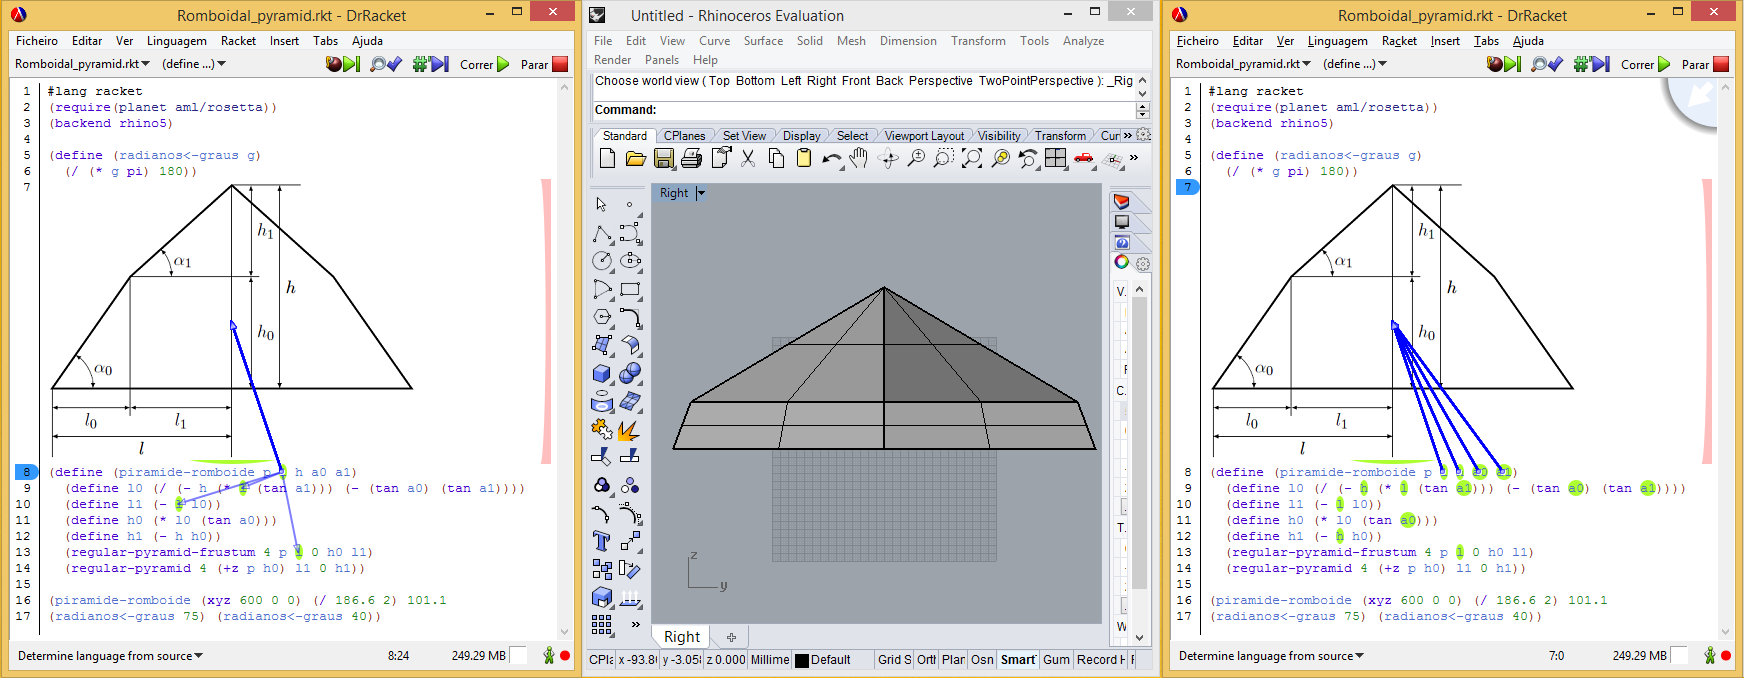
\includegraphics[scale=0.26]{img/rosetta2}
    \caption{Traceability with sketches. On the left, a parameter of the function was selected and an dark blue arrow was traced in the code. In the center is the generated model. On the right, the image was pointed and the parameters associated to the image were highlighted.}
  \label{fig:trace}
\end{figure}